\section{Handling Intermittent Electricity Generation}
\textit{Patrick Shower}

\subsection{Introduction}

In this part of the policy recommendation, we consider a very fundamental 
question relating to increased penetration of solar energy: Can today's
demonstrated energy storage solutions effectively and economically deliver
power to federal buildings as needed, given the intermittent nature of solar
power generation? The answer to this question is far from straightforward.
Federal buildings exist in a wide array of climates and have variable energy
needs. An energy storage scheme that works for a military installation in New
Mexico might not be ideal for a post office in Maine.

Thus, energy storage solutions must be assessed both in terms of the power
capacity required by the buildings they serve and the prevalence of sunlight at
their location. In addition, factors such as limited space, required
responsiveness, and resilience under environmental stressors should be
considered. In certain conditions, one or more of these factors may be critical
in deciding which storage solution, if any, is most applicable.

To answer the stated question, we first present the most promising energy
storage technologies that are widely considered ``demonstrated''. A basic
description of each storage technology is given, along with an economic
assessment of capitol, labor, and upkeep costs associated with utilizing it.
Its reliability in terms of efficiency, lifetime, and environmental sensitivity
is also analyzed. Then, specific recommendations for storage technology are
offered as a function of environment and required storage capacity. Finally, we
discuss how well the proposed solutions address the stated challenge of
intermittent generation and compare them to solutions that do not involve
energy storage.

\subsection{Proposed Solutions}

The problem of intermittent energy production is not a new one. Over the
decades, interest in renewable energy has sparked the development of storage
mechanisms operating on several physical principles (see Figure 1 below).

\begin{figure}
\begin{center}
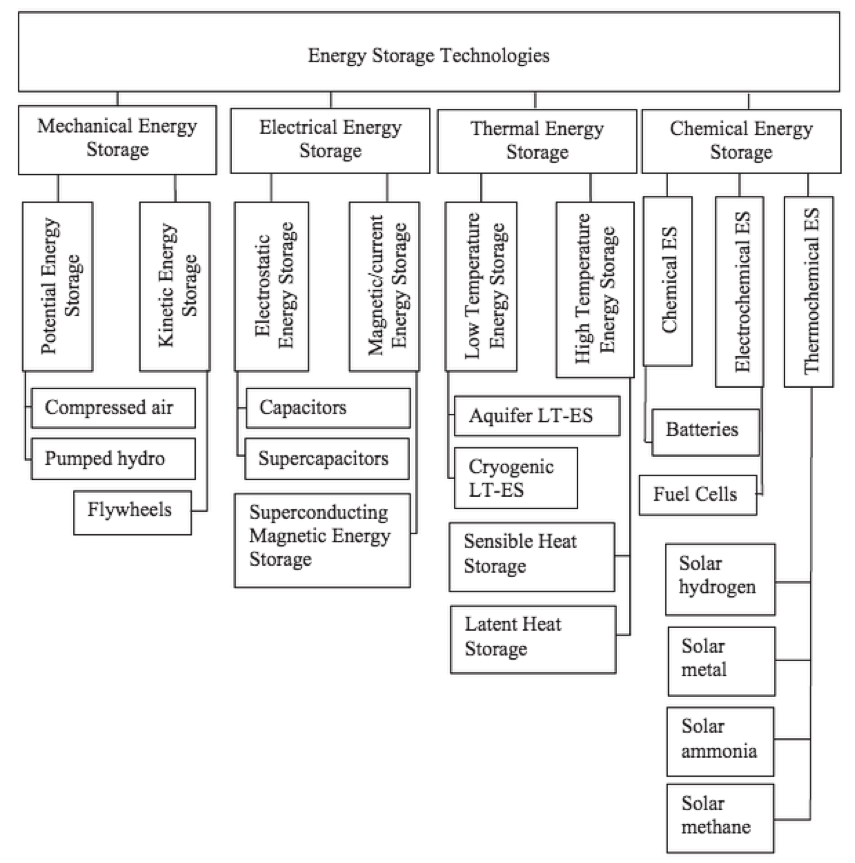
\includegraphics[scale=1.0]{pics/PatrickFigure1.png}
\caption{An impressive variety of energy storage mechanism have been studied in
parallel to the development of renewable energy generation.[1] }
\label{p1}
\end{center}
\end{figure}

Of these solutions, Compressed Air, Pumped Hydro, Flywheels,
Capacitors/Supercapacitors, Sensible Heat Storages, and Batteries are
considered ready to deploy on a commercial scale.[1] Each of these technologies
is evaluated below for their usefulness in storing energy generated by
photovoltaics for use in government buildings. In order to give the reader a
sense of scale when considering the power capacities of these technologies, the
following information is reported by the Energy Information Agency:
\begin{itemize}
\item There are a total of 84,000 government buildings in the country, together
consuming approximately .093 Quadrillion BTU annually.
\item Therefore, an average government building uses an average of .037 MW
throughout a 24-hour period.
\item There are 41,000 Government Buildings that consume between .00208 MW and
.0104 MW on average.
\item There are 35,000 Government Buildings that consume between .0104 MW and
.104 MW on average.
\item There are 5,000 Government Building that consume more than .104 MW, and
the largest government building by square footage, the Pentagon, consumes roughly
12.6 MW.[2]
\end{itemize}

For each technology, three critical metrics are listed. Capacity refers to the
power that the technologies can continuously discharge, with upper and lower
bounds determined both by technological limitations and efficiencies of scale.
Round trip efficiency refers to the amount of electrical energy the system can
discharge as a percentage of the energy it is charged with. Capital refers to
the initial cost of equipment per unit energy of storage. These criteria
represent a snapshot of how effective and economical a given storage technology
is for a particular application.

\subsubsection{Compressed Air}
\textbf{Capacity: 3-15 MW}

\noindent\textbf{Round Trip Efficiency: 50 \%}

\noindent\textbf{Capital: 100 \$/kWh}

Compressed Air Energy Storage (CAES) operates on the principle of
pressure-volume energy, which is converted to kinetic energy upon expansion in
a turbine. Below ground CAES has been demonstrated in Germany and the US on the
utility scale, being linked to a 290 MW and 110 MW plant, respectively. The
compressed air can be stored either underground - which requires locating a
suitable cavern - or above ground in man-made pressure vessels. The statistics
given are for above ground storage, more applicable in the case of federal
buildings because they could be implemented in any location with enough space
for a compressed air tank, regardless of geology.

Compressed air has been shown to be economical and reliable on the utility
scale, and represents a relatively modest capital investment as compared to
more technologically advanced solutions. However, its applications to single
federal buildings is likely limited due to its lower bound of power capacity, 3
MW. While CAES systems as small as 25 W have been produced on the laboratory
scale, these have not been rigorously evaluated by industry and will not likely
be deployable in the timeframe this policy concerns. Only the largest federal
buildings, or perhaps connected networks of buildings, would be effectively
served by this solution.

\subsubsection{Pumped hydro storage}
\textbf{Capacity: 100-5000 MW}

\noindent\textbf{Round Trip Efficiency: 75 - 85 \%}

\noindent\textbf{Capital: 100 \$/kWh}

Pumped hydro storage is another demonstrated technology that is known to be
effective at the utility scale. However, due to the difference in elevation
required (hydroelectric power generation is very dependent on the height or
``head'' of the water above the turbine, to the 3/2 power to be precise) this
technology is much more difficult to scale down, and thus would not be
applicable to any system with a capacity less than 100 MW. Since this excludes
federal buildings, pumped hydro storage is not applicable to the policy in
question.

\subsubsection{Flywheels}
\textbf{Capacity: .25 MW}

\noindent\textbf{Round Trip Efficiency: 93 - 95 \%}

\noindent\textbf{Capital: 5000 \$/kWh}

A flywheel is a mechanism that stores kinetic energy in a rotating mass. The
most recent iterations of this technology involve a carbon-fiber wheel that
rotates on a low friction or magnetic levitation bearing for minimal energy
loss to friction. As excess energy is generated, a motor propels the flywheel,
increasing the angular momentum of the system. As energy is required, the motor
acts as a generator to convert this momentum to electricity. This technology
has been proven effective in smoothing out intermittent power production,
primarily in wind systems. An individual flywheel can only sustain discharges
for times up to 15 minutes or so, and standby losses (the flywheel losing
energy over time due to friction) limit the effective duration of energy
storage.  This is a technologically advanced solution, and the up-front capitol
costs are the greatest of any of the solutions discusses. The merits of this
technology - its proven 20 year lifespan and its ability to charge and
discharge more rapidly than most other storage solutions - mean there are niche
applications could stand to benefit from the large investment.


\subsubsection{Supercapacitors}
\textbf{Capacity: 0-.3 MW}

\noindent\textbf{Round Trip Efficiency: 90 - 95 \%}

\noindent\textbf{Capital: 2000 \$/kWh}

Unlike the above solutions that necessitate the conversion of electrical energy
to mechanical energy and back, supercapacitors operate by storing energy in an
electric field. They entail a lower capitol expense than flywheels while
maintaining a similar efficiency and capacity. They also are expected to have a
20 year lifespan with continuous charging and discharging, and are able to
operate between -40$\degree$F and 160$\degree$F, encompassing temperatures they
would likely be exposed to in the US. Since the total energy storage of a supercapacitor is:
\begin{equation}
W_{eff}=\frac{C}{2}*(V^2_{max}-V^2_{min})
\end{equation}

The storage necessary can be scaled as needed for the application by varying
capacitance (C). One drawback is that supercapacitors can only effectively
discharge for one hour, so it is unlikely that a single supercapacitor would be
able to serve the needs of a federal building. The utilization of
supercapacitors requires advanced power electronics, which add complication and
expense. Ultimately, their hardiness can justify this expense in extreme
environments where cheaper forms of storage aren't reliable.


\subsubsection{Thermal Storage}
\textbf{Capacity: 0-60 MW}

\noindent\textbf{Round Trip Efficiency: 30-60 \%} 

\noindent\textbf{Capital: 100 \$/kWh}

The thermal storage of energy can take several forms. It can operate at high
temperatures or cryogenic temperatures, and can store energy in the form of
latent heat of phase transformation or sensible heat stored in a single-phase
medium. High temperature, sensible heat storage systems are the most developed,
and can be based around materials such as graphite, hot rocks, and molten salt.
A heat pump is used to input thermal energy to these media, and the energy is
discharged to produce supercritical steam in a conventional steam generator.
This method requires a lower investment in terms of development and
manufacturing than other thermal storage methods.
 
As compared to flywheels and supercapacitors, thermal storage can have very
long sustained run times, up to 24 hours or more. In relation to powering
federal buildings, this means that fewer thermal storage systems would be
required to power the structure over extended periods of solar deficit. A
molten salt storage scheme was shown to be effective in the Solar Two project.
In Solar Two, molten salt was used as a thermal storage mechanism, and 99\% the
thermal energy was effectively converted to electricity, as compared to
generating electricity directly from the heat of the solar input.[3]
Furthermore, while the use of this technology requires the development of a
physical storage system, it has been demonstrated that such systems can be made
on ``roof-top scale'' for ``micro-utilities'', and these systems are characterized
by energy densities similar to lithium-ion batteries.

\subsubsection{Batteries}
\textbf{Capacity: 0-40 MW}

\noindent\textbf{Round Trip Efficiency: 60 - 90 \%}

\noindent\textbf{Capital: 400-2500 \$/kWh}

A wide variety of batteries have been developed for energy storage
applications. Some of these include, in order of increasing round-trip
efficiency, Ni-Cd, Pb-Acid, Na-S, and Li-ion batteries. In general, they are
expected to be functional for between 2000 and 4500 charge-discharge cycles, or
between 5 and 13 years if they undergo one cycle per day. This is about half of
the expected lifetime of storage systems, so there is an increased long-term
investment related to system upkeep. Furthermore, all the batteries listed
require either heating or air conditioning to maintain functionality. If
they're utilized in an environment that would require a significant amount of
energy to maintain operating temperature, this is yet another associated expense.

One advantage that batteries present is their energy density. Of the solutions
discussed so far, thermal energy storage has the greatest energy density, at 80
- 200 watt hours per kilogram. Li-ion batteries have a similar energy density
(75 - 200 Wh/kg) while Na-S batteries have an increased energy density (150-240
Wh/kg), and both are approximately twice as energy efficient as thermal
storage.

\subsection{Evaluation}
The necessary storage capacity of any given building was estimated under a
``worst case scenario'' set of assumptions. Namely these are:
That the buildings will run exclusively off of generated photovoltaic power?

The evaluation of these technologies was based on two central aspects. First,
the storage demand for any given federal building was estimated based on its
average power capacity and the ability of its environment to support solar
power. Second, the total cost of installing and operating each of the storage
systems listed for 20 years was estimated as a function of storage capacity
installed. Thus, the lowest-cost solution for any given capacity can be
indicated. Third, special considerations that may impact the choice of a
storage technology, such as climate, required responsiveness, and limited
space, were identified and matched with an appropriate technology.

\subsubsection{Estimating storage demand}

To estimate the needed storage demand, the problem to be solved must first be
defined. In this case, it's not so much a matter of evening solar output vary
from day to day, but evening it out over the course of the day. The base-line
utilities know what the basic load profile will look like depending on the
region and the time of year. If they can predict 24 hours in advance how much
solar power will need to be compensated for, they can ensure that the total
energy demand is met. The problem comes when, for instance, a sunny day is
expected and a cloudy day occurs instead. In this case, the base-line utilities
can be sluggish in their response. If the output of photovoltaic sources on the
grid were to drop by more than approximately 5\% per hour, the utilities would
not be able to respond effectively and power demand would not be met. This corresponds to:

.037 MW per building, 28 buildings per county on average, 5\% of X\% (capacity)
of this product is .052*X MW/hour.

In a worst case scenario, the utilities will have planned on a perfectly sunny
day, with a output profile shown by a solid blue line in figure 2 below. At
some point during the day, PV output will drop to zero and energy storage will
have to compensate for the rest of the day. If the output of the PV/Storage
system drops by 5\% each hour until the projected power output is met again it,
the output of the PV array would look like the blue dashed line below and the
storage output would look like the red output in fig. \ref{p2}

\begin{figure}
\begin{center}
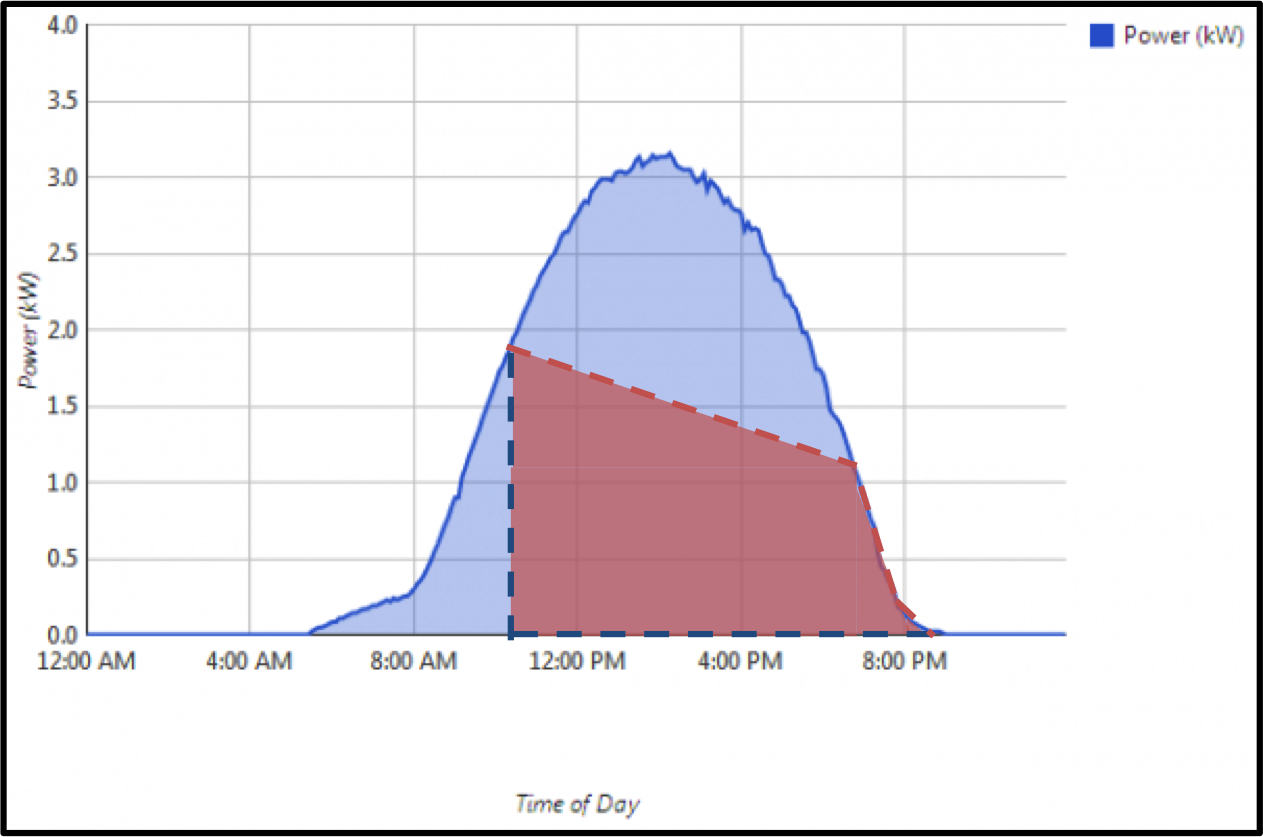
\includegraphics[scale=0.6]{pics/PatrickFigure2.png}
\caption{Storage output.}
\label{p2}
\end{center}
\end{figure}

Therefore, the area under the dashed red line, hightlighted in red, represents
the total energy storage required to get through the day. For such a geometry,
the maximum area under the curve will be roughly 56\% of the total energy
capacity of the PV system, the area under the solid blue line. In terms of
energy storage, this means that approximately 56\% of a system's daily output
must be stored to maintain the integrity of the grid in a ``worst case scenario''
day.

According to the Stefan-Boltzmann law describing radiation from a blackbody:
\begin{equation}
j^* = \sigma T^4
\end{equation}

Where T is absolute temperature [K], $\sigma$ is a constant equal to 5.670*10-8
$\frac{W}{m^2*K^4}$, and $j^*$ is the energy radiated per unit surface area of
the blackbody.
Assuming a steady state where incoming flux to the blackbody is equal to
outgoing flux and accounting for the albedo of the earth:
\begin{equation}
T={(\frac{j^*}{\sigma})}^{1/4}=(\frac{j_o(1-albedo)}{\sigma})^{1/4}
\end{equation}

Where jo is the flux, and albedo of the earth is approximately 0.3. Solving for
incoming flux:
\begin{equation}
j_o=T^4*\sigma*1.429
\end{equation}

If flux is proportional to the output of a photovoltaic array under that flux:
\begin{equation}
\frac{j_{o,1}}{j_{o,2}}=\frac{output_1}{output_2}=\frac{T_1^4}{T_2^4}
\end{equation}
If output2 is assumed to be on a cloudy day (worst case scenario), then a more
accurate relationship would be:
\begin{equation}
\frac{j_{o,1}}{0.4j_{o,2}}=\frac{output_1}{output_2}=\frac{T_1^4}{0.4T_2^4}
\end{equation}
\begin{equation}
\frac{output_1}{output_2}=\frac{T_1^4}{0.4T_2^4}
\end{equation}

Since solar panels can only utilize 40\% of diffuse irradiation. If we want a
97.8\% chance that there will be enough storage capacity on any given day, we
can find the percentage in output that needs to be stored. Assuming that T1 is
the average temperature of the lower 48 states, 284.6 K, and that output1 is
the maximum output of any given day.

\begin{equation}
\begin{aligned}
\frac{output_{max}-(\text{PV output}_2+\text{storage output})}{output_{max}} &=
\\
1-.4\frac{(284.6[K]-2*stddev)^4}{(284.6[K])^4}-\frac{storage}{output_{max}}
&=.45
\\
\end{aligned}
\end{equation}
 
where ``stddev'' is the standard deviation of
temperature at the building location, which can be taken from fig. \ref{p3}
below.

\begin{figure}
\begin{center}
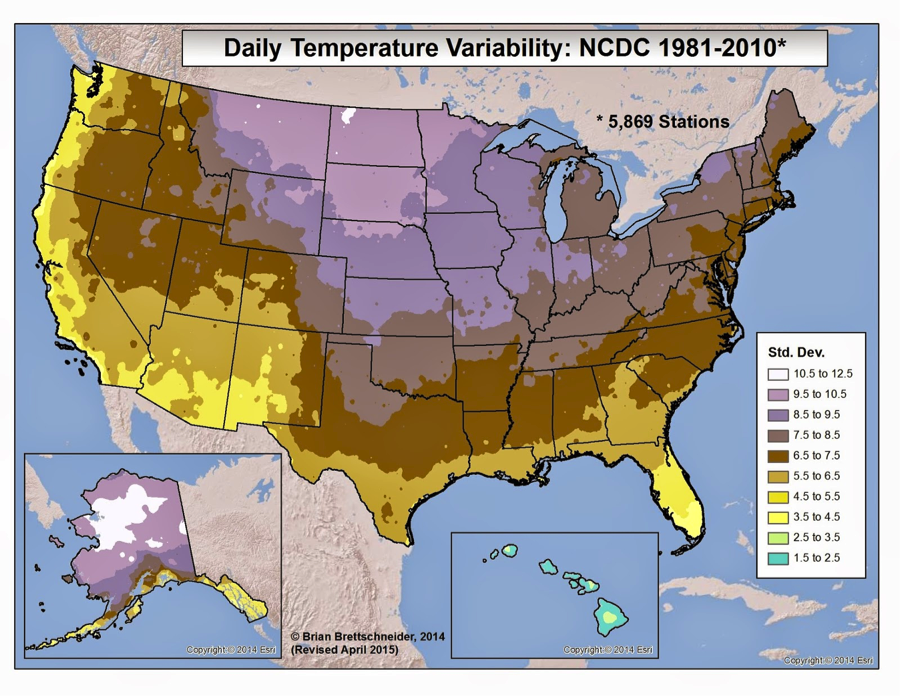
\includegraphics[scale=1.0]{pics/PatrickFigure3.png}
\caption{Daily Temperature Variability}
\label{p3}
\end{center}
\end{figure}

Solving for the necessary storage as percent of capacity:
\begin{equation}
.55-.4\frac{(284.6[K]-2*stddev)^4}{(284.6[K])^4}=\frac{storage}{output_{max}}
\end{equation}

The amount of storage needed to handle the worst case scenario day one and the
second worst case scenario day two will also depend on whether or not the
storage will be able to recharge in the interim. This is effectively a function
of how likely a sunny day is at the building site. At any given location on the
globe, there are 4383 hours of daytime (and 4383 hours of night) per year.
Assuming that 5\% of the PV energy generated is diverted to storage during any
given hour, approximately 11 hours would be needed to recharge the storage
system that supports 56\% of the total daily demand. In a worst case scenario
(at the northern fringe of the continental US on the winter solstice), there
are approximately 9 hours between sunrise and sunset. So at most, 45\% of daily
capacity could be stored in such a scenario. This means that at least an
additional 10\% of daily capacity would have to be accounted for in pre-stored
energy, and 55\% at most. The calculation of average hours of sunlight in 9
hours of daytime is fairly straightforward:

\begin{equation}
hrs_{sun,avg}=\frac{hrs_{sun,annual}}{4383 [hrs]}*9 [hrs]
\end{equation}

Using this expression to estimate the percentage of daily capacity that may be
expected to regenerate:

\begin{figure}
\begin{center}
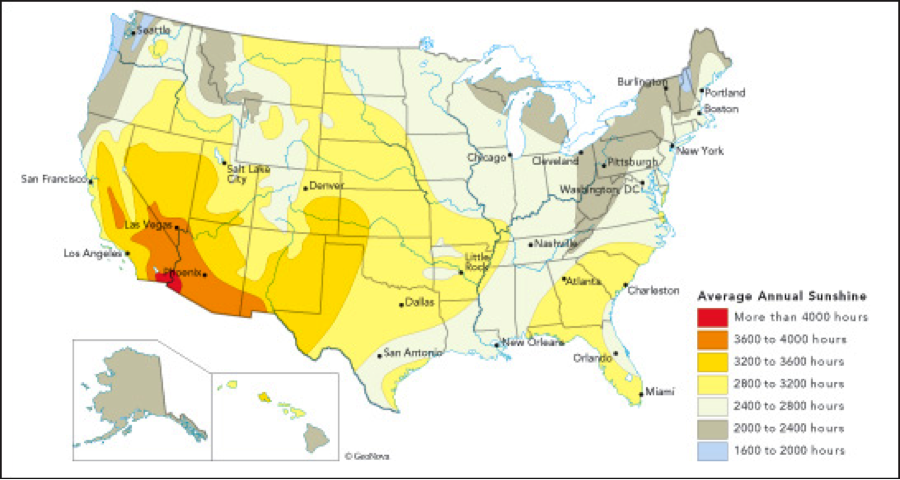
\includegraphics[scale=1.0]{pics/PatrickFigure4.png}
\caption{Average Annual Sunshine}
\label{p4}
\end{center}
\end{figure}

\begin{equation}
\frac{storage_{required}-storage_{regenerated}}{output_{max}} =
.55-.05*\frac{hrs_{sun,annual}}{4383} [hrs]*9
\end{equation}

Thus, calculating the total storage needed for this worst case scenario:
\begin{equation}
\begin{aligned}
\frac{Storage}{output_{max}}&=storage_{Day1}+storage_{Day2}-expected
regeneration
\\
&=.55+.55-.4\frac{(284.6[K]-2*stddev)^4}{(284.6[K])^4}-.05*\frac{hrs_{sun,annual}}{4383
[hrs]}*9 [hrs] \\
&=1.1-.4\frac{(284.6[K]-2*stddev)^4}{(284.6
[K])^4}-.45*\frac{hrs_{sun,annual}}{4383}  \\
\end{aligned}
\end{equation}
\begin{equation}
Storage=output_{max}(1.1-.4\frac{(284.6[K]-2*stddev)^4}{(284.6
[K])^4}-.45*\frac{hrs_{sun,annual}}{4383})
\end{equation}

Capturing the influence of the building location on the necessary storage capacity:
\begin{equation}
\text{Environmental Factor}=1.1-.4\frac{(284.6[K]-2*T_{stddev})^4}{(284.6
[K])^4}-.45*\frac{hrs_{sun,annual}}{4383})
\end{equation}

\subsubsection{Evaluation of cost}

The average service life required for photovoltaic panels to pay themselves off
is 15-25 years. Conveniently, all of the storage mechanisms listed will last 20
years, excepting batteries which last an average of 10 years or so with daily
cycling. Given these facts, 20 years was chosen as a time frame over which to
estimate the cost of capital, installation, and maintenance for each energy
storage solution.

\begin{figure}
\begin{center}
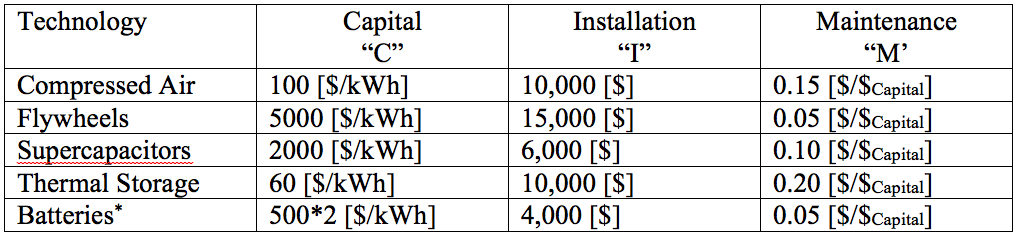
\includegraphics[scale=0.3]{pics/PatrickTable0.png}
\caption{Based on Sodium-Sulfur batteries, which we judged to be the most
reliable, efficient, and suitable in this application.}
\label{patrickTable0}
\end{center}
\end{figure}

So, the 20 year cost can be calculated as:
\begin{equation}
\begin{aligned}
Total cost&=Capital+Installation+Maintenence\\
Total cost&=(C[\frac{\$}{kWh}](1+M[\frac{\$}{\$}])*Capacity[kWh])+I\\
\end{aligned}
\end{equation}

This function is graphed below for each of the five proposed storage
technologies. Note that flywheels and compressed air both have a minimum
threshold capacity, and are plotted only over the capacity range in which they
are feasible.

\begin{figure}
\begin{center}
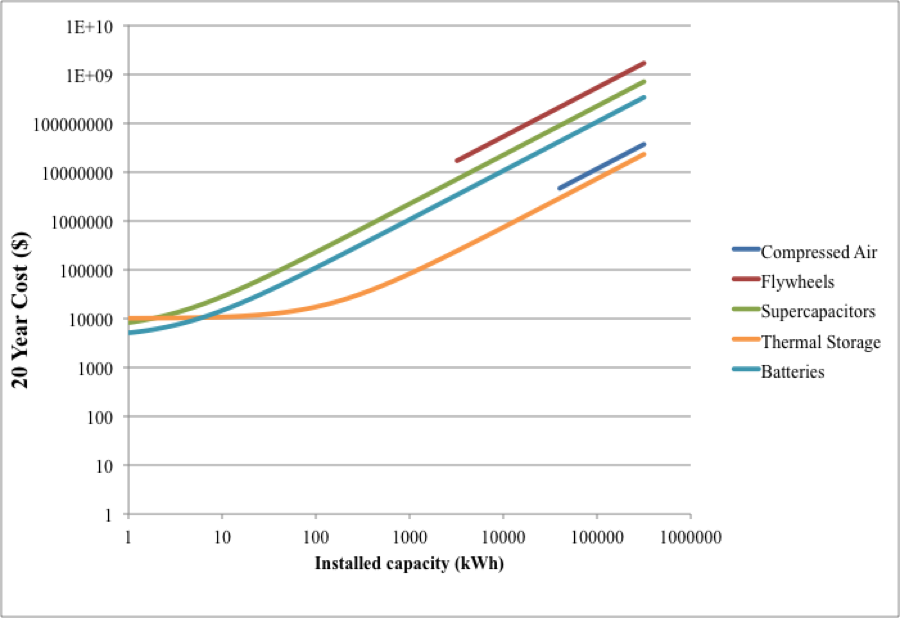
\includegraphics[scale=1.0]{pics/PatrickFigure5.png}
\caption{20 year cost}
\label{p5}
\end{center}
\end{figure}

Thus, Sodium-Sulfur batteries are expected to be most affordable for storage
capacities below 7 kWh, and thermal storage for capacities above 7 kWh. Using
this data, the most economic storage mechanism can be identified as a function
of environmental factor and the installed PV capacity required by the policy (a
certain percentage of total energy demand, depending on the date of
construction or retrofitting). These results are summarized below:

\begin{figure}
\begin{center}
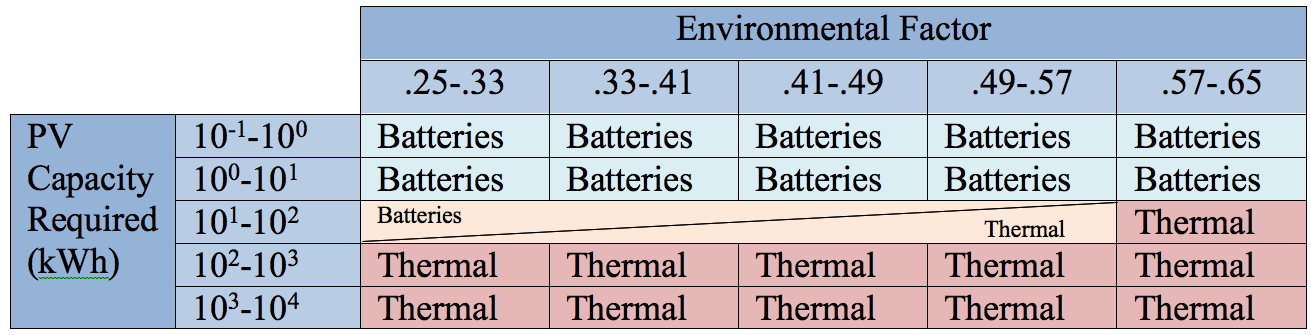
\includegraphics[scale=0.3]{pics/PatrickTable1.png}
\caption{Environmental Factors}
\label{patrickTable1}
\end{center}
\end{figure}

If this is applied to Greve Hall, with a daily energy consumption of $=4.285*103
kWh$ and an environmental factor, E, 
\begin{equation}
\begin{aligned}
E &=(1.1-.4\frac{(284.6[K]-2*7.2)^4}{(284.6[K])^4}-.45*\frac{2400}{4383})\\
&=.56681\\
\end{aligned}
\end{equation} 
Indicating that a thermal storage system would be the most affordable solution.

Of course, not all storage scenarios can be fully described by two numbers. In
some cases, there will be particular demands or constraints that may
necessitate the use of a more expensive storage technology. These include:
\begin{itemize}
\item Situations in which the photovoltaic array represents a very significant
portion of the total grid input, and the ability of the storage system to
compensate for PV loss within a few milliseconds is important. In this case,
flywheels have been demonstrated to have very quick ramp-up and ramp-down rates
in conjunction with solar systems.
\item Situations in which temperature extremes are expected and it's not
feasible to control the storage system's environment. Supercapacitors stand out their abity
to operate between -40$\degree$F and 160$\degree$F for long cycle lifetimes.
\end{itemize}

\subsection{Conclusions}

Can today's demonstrated energy storage solutions effectively and economically
deliver power to federal buildings as needed, given the intermittent nature of
solar power generation? We believe that the data here presented evidences that
they can. For any given combination of environment and PV capacity, one of two
energy storage solutions is the most viable. This elegant result will simplify
the installation of the PV array/storage system and allow costs to be
minimized. In terms of cost, it is worth noting that the cost of thermal energy
storage is approximately \$300 per kW, and as low as \$300 per kW in battery
systems. Given that the photovoltaic arrays here discussed cost on the order of
\$2,000 per kW, this additional cost is non-negligible, but extremely reasonable
to ensure the reliability of the grid.

Furthermore, while alternative solutions to intermittency could be established,
such as on-site generation using existing natural gas sources, this policies
commitment to carbon neutrality heavily favors the philosophy of energy
storage. In addition to stand-alone storage systems, rechargeable electric
vehicles could also fill the role of intermittency mitigation. This possibility
is discussed in another section.
